%\documentclass[xetex,aspectratio=169,handout,notes=show]{beamer}
\documentclass[xetex,aspectratio=169]{beamer}
\usepackage{amsmath}
\usepackage{amsthm}

\usepackage{minted}

%\usepackage{listings}

\usepackage{xcolor}
\hypersetup{
    colorlinks=true,
    linkcolor={red!60!black},
    citecolor={red!60!black},
    urlcolor={red!60!black}
}

\newcommand{\ZZ}{\mathbb{Z}}
\newcommand{\FF}{\mathbb{F}}
\DeclareMathOperator{\id}{id}

\newcommand{\Term}[2]{{\textbf{#1. }}{#2}}
\newcommand{\uniformsample}{\xleftarrow\$}

\usetheme[progressbar=frametitle]{metropolis}

\title{\mbox{Fast, Safe, Pure-Rust Elliptic Curve Cryptography}}
\author{Isis Lovecruft} %/ Henry de Valence}
%\institute{}
\date{Noisebridge 10th Anniversary \\ September 2017}

\begin{document}
\maketitle

\begin{frame}
  \frametitle{Introductions}

  \begin{itemize}
    \item<2-> This talk is for those with light familiarity with Rust.
    \item<3-> It \emph{isn't} aimed at cryptographers.
    %% no math no worry
    \item<4-> Don't worry! We'll cover the basic terminology, and --- with a tad
      of high-school level algebra --- you should be able to follow along just
      fine.
    \item<5-> If not, still don't worry! All questions are welcome, and if
      you're shy please feel free to talk to us privately afterwards, either in
      person or online.
  \end{itemize}
\end{frame}

\begin{frame}
  \frametitle{Overview}
  \tableofcontents
\end{frame}

\section{What is \texttt{curve25519-dalek}?}

  \begin{frame}
    \frametitle{Anatomy of an elliptic curve cryptography implementation}
    
    \begin{columns}[c]
      \column{0.5\textwidth}
    \begin{tabular}{|r|l|}
      \hline
      \multicolumn{2}{|c|}{Applications} \\
      \hline \hline
      Protocol & Protocol-specific library \\
      \cline{2-2}
      Group & \\
      Elliptic Curve & \texttt{curve25519-dalek} \\
      Finite Field & \\
      \hline \hline
      \multicolumn{2}{|c|}{CPU} \\
      \hline
    \end{tabular}
      \column{0.5\textwidth}
      
      \visible<2->{\alert{Protocol}: a specific cryptographic operation, such as a signature, a zero-knowledge proof, etc.}
      
      \visible<3->{\alert{Group}: an abstract mathematical structure (like a trait) implemented concretely by an\ldots}

      \visible<4->{\alert{Elliptic Curve}: a set of points satisfying certain equations defined over a\ldots}

      \visible<5->{\alert{Finite Field}: usually, integers modulo a prime $p$.}
    \end{columns}
    
    \visible<6->{
    Our implementation was originally based on Adam Langley's \texttt{ed25519} Go code, which was in turn based on the reference \texttt{ref10} implementation.
    }
  \end{frame}

  \begin{frame}
    \frametitle{Historical Implementations}

    In order to talk about what \texttt{curve25519-dalek} is, and why we made
    it, it's important to revisit other elliptic curve libraries, their designs,
    and common problems.

  \end{frame}


  \begin{frame}
    \frametitle{Historical Implementations: Part I}

    Other elliptic curve libraries tend to have no separation between
    implementations of the field, curve, and group, and the protocols sitting on
    top of them.

    \pause This causes several immediate issues:

    {\small
    \begin{itemize}
      \item<3-> Idiosyncracies in the lower-level pieces of the implementation
        carry over into idiosyncracies in the protocol.
      \item<4-> Assumptions about how these lower-level pieces will be used
        aren't necessarily correct if someone wanted to reuse the code to
        implement a different protocol.
      \item<5-> Excessive copy-pasta with minor tweaks by other cryptographers
        (worsened by the fact that some cryptographers think that
        releasing unsigned tarballs of their implementations \emph{inside} another
        tarball of a benchmarking suite is somehow an appropriate software
        distribution mechanism).
    \end{itemize}
    }
  \end{frame}


  \begin{frame}
    \frametitle{Historical Implementations: Part I (cont.)}

    This leads to large, monolithic codebases which are idiosyncratic,
    incompatible with one another, and highly specialised to perform only the
    single protocol they implement (usually, a signature scheme or
    Diffie-Hellman key exchange).

    The modus operandi for implementing cryptographic software is
    writing microarchitecture-optimised, \emph{artisinal assembly},
    with the purported goals of lower clock cycles and
    constantimedness. (However the neither goal is guaranteed, as
    we'll see later.)

  \end{frame}


%  \begin{frame}
%    \frametitle{Historical Implementations: Part II}
%
%    There are worse problems.
%
%    \pause Cryptographers aim to protect against \emph{side-channel attacks} by
%    writing constant-time code.
%
%    \pause Traditionally, due to variations in implementations of C compilers
%    (and other high- or higher-level languages), many cryptographers who study
%    constant-timedness insist that writing assembly is the only solution. (This
%    is still not a solution, cf. non-constant-timedness of the MUL operation on
%    PowerPC.)
%
%    \pause This has led to many of these monolithic, idiosyncratic,
%    protocol-specific implementations being written in \emph{artisanal assembly}.
%
%  \end{frame}


 \begin{frame}
   \frametitle{Historical Implementations: Part II}

   \emph{There's still worse.} \pause One cryptographer proclaimed the
   following, unspecified, undocumented, not-fully-implemented macro
   ``language'' for generating artisanal assembly to be…

   \pause \begin{tabular}{ccc}
     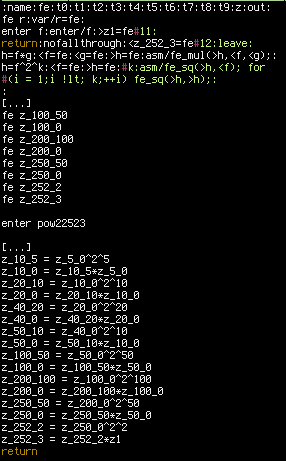
\includegraphics[height=6cm]{quackery-before.jpg} &
                     {\LARGE $\Rightarrow$} &
     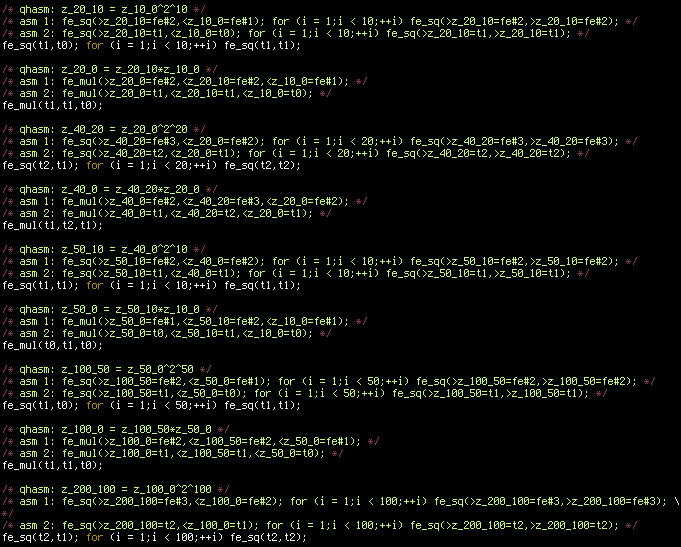
\includegraphics[height=6cm]{quackery-after.jpg}
   \end{tabular}
 \end{frame}


 %% https://news.ycombinator.com/item?id=9397169
 {
   \usebackgroundtemplate{%
     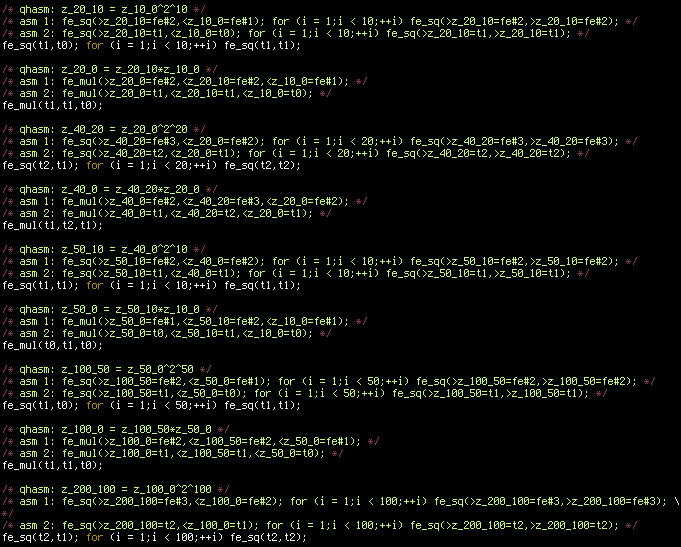
\includegraphics[width=\paperwidth]{quackery-after}}
   \begin{frame}[plain]
     \frametitle{``THE DEATH OF OPTIMISING COMPILERS''}
   \end{frame}
 }

  \begin{frame}
    \frametitle{Historical Implementations: Part II (cont.)}

    \emph{And there's still worse.}

    \pause In major, widely-used, cryptographic libraries:

    \begin{itemize}
      \item<2-> Using C pointer arithmetic \emph{to index an array}.  In C,
        array indexing works both ways, e.g. \texttt{a[5] == 5[a]}. In this case
        they were doing \texttt{a[p+5]} (\texttt{== a+p[5] == 5[a+p]}).
      \item<3-> Overflowing signed integers in C and expecting the behaviour to
        be sane/similar across platforms and varying compilers.
      \item<4-> Using untyped integer arrays (e.g. \texttt{[u8; 32]}) as
        canonical, external representation for mathematically fundamentally
        incompatible types (e.g. points and numbers)
      \item<5-> Using pointer arithmetic to determine both the size and location
        of a write buffer.
      \item<6-> \emph{I can keep going.}
    \end{itemize}
  \end{frame}


  \begin{frame}
    \frametitle{Design Goals of \texttt{curve25519-dalek}}

    \begin{itemize}
      \item<1-> Usability
      \item<2-> Versatility %% for both common and exotic protocol implementation
      \item<3-> Safety
        {\small
        \begin{itemize}
          \item<4-> Memory Safety
          \item<5-> Type Safety
          \item<6-> Overflow/Underflow Detection
            % XXX more kinds of safety?
        \end{itemize}
        }
      \item<7-> Readability \visible<9->{ …which implies}
        {\small
        \begin{itemize}
          \item<8-> Explicitness
        \end{itemize}
        }
      \item<10-> Auditability
    \end{itemize}

    \visible<11->{These are all things we would get from a higher-level, memory-safe,
    strongly-typed, polymorphic programming language,}

    \visible<12->{a.k.a} \visible<13->{Rust.}

  \end{frame}


%% \section{Implementing low-level arithmetic in Rust}
%% 
%%   \begin{frame}
%%     \frametitle{Example: implementing multiplication in $\FF_p$, $p = 2^{255} - 19$}
%%     
%%     Let's jump down to the lowest abstraction layer: using primitive
%% types to implement field arithmetic.
%%     
%%     \pause Specifically: how can we implement multiplication of two
%% integers modulo $p = 2^{255} - 19$, using only the primitive
%% operations provided by the CPU?
%% 
%%     \pause Two questions:
%%     \begin{itemize}
%%     \item<4-> What are the primitive operations?
%%     \item<5-> What does multiplication in $\FF_p$ look like?
%%     \end{itemize}
%%   \end{frame}
%%   
%%   \begin{frame}
%%     \frametitle{Multiplication modes}
%%     Primitive types have a fixed size: \texttt{u8}, \texttt{i8}, \ldots, \texttt{u64}, \texttt{i64}, etc., but numbers get bigger when you multiply them.  What happens?
%%     
%%     \pause
%%     \begin{enumerate}
%%     \item<3-> Error on overflow (\alert{debug}): \texttt{8u8 * 40u8 == panic!()}
%%     \item<4-> Wrapping arithmetic (\alert{release}): \texttt{8u8 * 40u8 == 64u8}
%%     \item<5-> Saturating arithmetic: \texttt{8u8 * 40u8 == 255u8}
%%     \item<6-> Widening arithmetic: \texttt{8u8 * 40u8 == 320u16}
%%     \end{enumerate}
%%     
%%     \visible<7->{
%%     Rust has intrinsics for 1, 2, and 3, and we can get 4 by writing 
%% 
%%     \texttt{(x as T) * (y as T)},
%% 
%%     where \texttt{T} is the next-wider type.
%%     }
%%    
%%   \end{frame}
%%   
%%   {
%%     \usebackgroundtemplate{%
%%       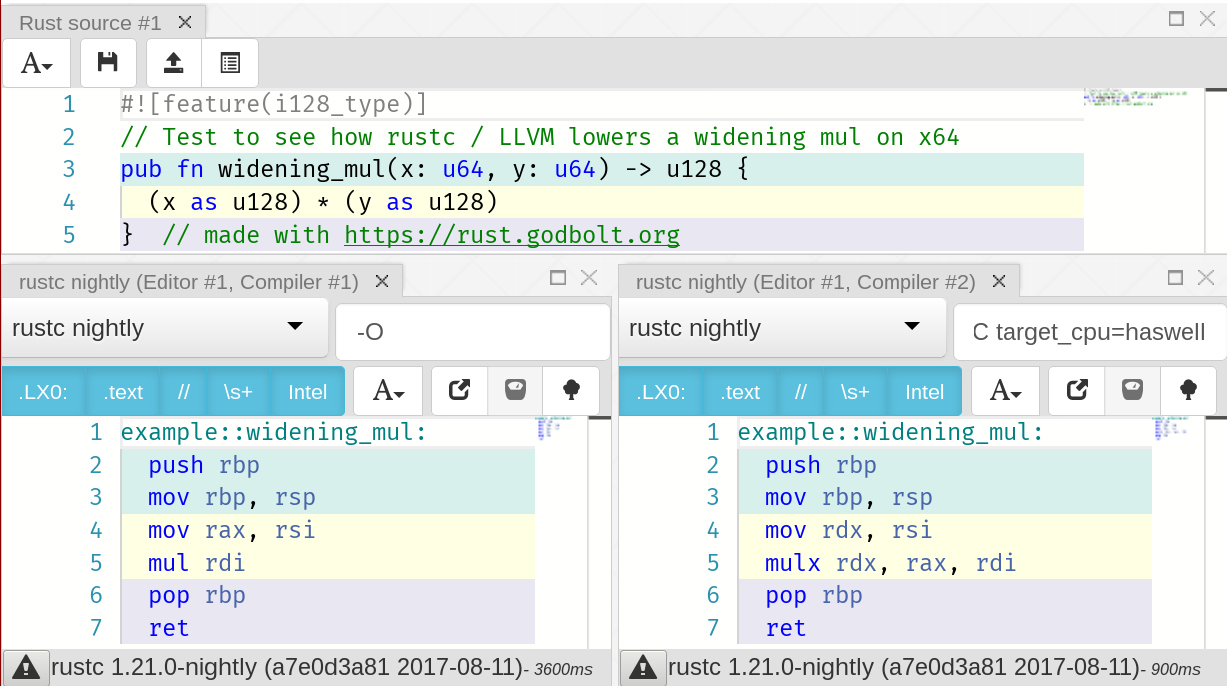
\includegraphics[width=\paperwidth]{rustc-widening-multiply-lowering.png}}
%%     \begin{frame}[plain]
%%       \frametitle{Lowering widening multiplication to assembly on x86-64}
%%     \end{frame}
%%   }
%%   
%%   \begin{frame}
%%     \frametitle{Radix-$2^{51}$ representation}
%%     
%%     The Ed25519 paper suggests using a ``radix-$2^{51}$'' representation.
%% 
%%     \pause What does this mean? It means we write numbers $x, y$ as
%%     \begin{align*}
%%       x &= x_0 + x_12^{51} + x_22^{102} + x_32^{153} + x_42^{204} \qquad 0 \leq x_i \le 2^{51} \\
%%       y &= y_0 + y_12^{51} + y_22^{102} + y_32^{153} + y_42^{204} \qquad 0 \leq y_i \le 2^{51} 
%%     \end{align*}
%%     
%%     \pause Since $2^{51} < 2^{64}$, we can write this as 
%% 
%%     \texttt{struct FieldElement64([u64;5])}
%%     
%%     and use the widening multiplication 
%% 
%%     \texttt{(x[i] as u128) * (y[j] as u128)}
%%     
%%     \end{frame}
%% 
%%    \begin{frame}
%%    \frametitle{Multiplication, part I}
%%     How do we multiply? Set $z = xy$. Then we can write down the coefficients of $z = z_0 + z_12^{51} + z_22^{102} + \ldots$
%%     %\begin{align*}
%%     %  z_0 &= x_0y_0 & & & &\\
%%     %  z_1 &= x_0y_1 +& x_1y_0 & & &\\
%%     %  z_2 &= x_0y_2 +& x_1y_1 +& x_2y_0 & &\\
%%     %  z_3 &= x_0y_3 +& x_1y_2 +& x_2y_1 +& x_3y_0 & \\
%%     %  z_4 &= x_0y_4 +& x_1y_3 +& x_2y_2 +& x_3y_1 +& x_4y_0 \\
%%     %  z_5 &=         & x_1y_4 +& x_2y_3 +& x_3y_2 +& x_4y_1 \\
%%     %  z_6 &=         &         & x_2y_4 +& x_3y_3 +& x_4y_2 \\
%%     %  z_7 &=         &         &         & x_3y_4 +& x_4y_3 \\
%%     %  z_8 &=         &         &         &         & x_4y_4 
%%     %\end{align*}
%%     \begin{align*}
%%       \visible<2->{ z_0 &= x_0y_0 & 1}\\
%%       \visible<3->{ z_1 &= x_0y_1 + x_1y_0 & 2^{51}}\\
%%       \visible<4->{ z_2 &= x_0y_2 + x_1y_1 + x_2y_0 & 2^{102}}\\
%%       \visible<5->{ z_3 &= x_0y_3 + x_1y_2 + x_2y_1 + x_3y_0  & 2^{153}}\\
%%       \visible<6->{ z_4 &= x_0y_4 + x_1y_3 + x_2y_2 + x_3y_1 + x_4y_0 & 2^{204}}\\
%%       \visible<7->{ z_5 &=          x_1y_4 + x_2y_3 + x_3y_2 + x_4y_1 & 2^{255}}\\
%%       \visible<8->{ z_6 &=                   x_2y_4 + x_3y_3 + x_4y_2 & 2^{306}}\\
%%       \visible<9->{ z_7 &=                            x_3y_4 + x_4y_3 & 2^{357}}\\
%%       \visible<10->{ z_8 &=                                     x_4y_4 & 2^{408}}
%%     \end{align*}
%%   \end{frame}
%% 
%%    \begin{frame}
%%    \frametitle{Multiplication, part II}
%% 
%%    Since $p = 2^{255} - 19$, we have $2^{255} \equiv 19 \pmod p$.  
%%    
%%    \pause This means that we can do inline reduction:
%%    {\small
%%    \begin{align*}
%%     % z &= z_0 + z_12^{51} + z_22^{102} + z_32^{153} + z_42^{204} \\
%%     %   &+ z_5 2^{255} + z_6 2^{306} + z_7 2^{357} + z_82^{408} \\
%%     % z &\equiv z_0 + z_12^{51} + z_22^{102} + z_32^{153} + z_42^{204} \\
%%     %   &+ z_5 19 + z_6 19 \cdot 2^{51} + z_7 19 \cdot 2^{102} + z_8 19 \cdot 2^{153} \qquad \pmod p
%%     &z_0 + z_12^{51} + z_22^{102} + z_32^{153} + z_42^{204} + z_5 2^{255} + z_6 2^{306} + z_7 2^{357} + z_82^{408} \\
%%     &\visible<3->{ \equiv (z_0 + 19z_5) + (z_1 + 19z_6)2^{51} + (z_2 + 19z_7)2^{102} + (z_3 + 19z_8) 2^{153} + z_42^{204}  \quad \pmod p}
%%    \end{align*}
%%    }
%%    \visible<4->{We can combine this with the formulas on the previous slide:}
%%     \begin{align*}
%%       \visible<5->{ z_0 &= x_0y_0 + 19( x_1y_4 + x_2y_3 + x_3y_2 + x_4y_1 )& 1}\\
%%       \visible<6->{ z_1 &= x_0y_1 + x_1y_0 + 19(x_2y_4 + x_3y_3 + x_4y_2 ) & 2^{51}}\\
%%       \visible<7->{ z_2 &= x_0y_2 + x_1y_1 + x_2y_0 + 19(x_3y_4 + x_4y_3 ) & 2^{102}}\\
%%       \visible<8->{ z_3 &= x_0y_3 + x_1y_2 + x_2y_1 + x_3y_0 + 19(x_4y_4) & 2^{153}}\\
%%       \visible<9->{ z_4 &= x_0y_4 + x_1y_3 + x_2y_2 + x_3y_1 + x_4y_0 & 2^{204}}\\
%%     \end{align*}
%%   \end{frame}
%%   
%% \begin{frame}[fragile]
%%     \frametitle{Rust implementation, part I}
%%     Let's write this in Rust:
%%     {\tiny
%%     \begin{minted}{rust}
%% impl<'a, 'b> Mul<&'b FieldElement64> for &'a FieldElement64 {
%%     type Output = FieldElement64;                            
%%     fn mul(self, _rhs: &'b FieldElement64) -> FieldElement64 {                                          
%%         #[inline(always)]                                                                               
%%         fn m(x: u64, y: u64) -> u128 { (x as u128) * (y as u128) }                                      
%%     
%%         // Alias self, _rhs for more readable formulas                                                  
%%         let a: &[u64; 5] = &self.0; let b: &[u64; 5] = &_rhs.0;                                         
%%         // 64-bit precomputations to avoid 128-bit multiplications                                      
%%         let b1_19 = b[1]*19; let b2_19 = b[2]*19; let b3_19 = b[3]*19; let b4_19 = b[4]*19;     
%%     
%%         // Multiply to get 128-bit coefficients of output                                               
%%         let c0 = m(a[0],b[0]) + m(a[4],b1_19) + m(a[3],b2_19) + m(a[2],b3_19) + m(a[1],b4_19);
%%         let c1 = m(a[1],b[0]) + m(a[0],b[1])  + m(a[4],b2_19) + m(a[3],b3_19) + m(a[2],b4_19);
%%         let c2 = m(a[2],b[0]) + m(a[1],b[1])  + m(a[0],b[2])  + m(a[4],b3_19) + m(a[3],b4_19);
%%         let c3 = m(a[3],b[0]) + m(a[2],b[1])  + m(a[1],b[2])  + m(a[0],b[3])  + m(a[4],b4_19);
%%         let c4 = m(a[4],b[0]) + m(a[3],b[1])  + m(a[2],b[2])  + m(a[1],b[3])  + m(a[0],b[4]); 
%%     \end{minted}
%%     }
%%     \pause However, the $c_i$ are too big: we want \texttt{u64}s, not \texttt{u128}s.
%% \end{frame}
%%   
%% \begin{frame}[fragile]
%%     \frametitle{Rust implementation, part II}
%%     To finish, we reduce the size of the coefficients by carrying their values upwards into higher coefficients:
%%     $(c_{i+1}, c_i) \leftarrow (c_{i+1} + \lfloor c_i / 2^{51} \rfloor, c_i \mod 2^{51})$
%%     \pause
%%     {\tiny
%%     \begin{minted}{rust}
%%         let low_51_bit_mask = (1u64 << 51) - 1;
%%         c1 +=  c0 >> 51;
%%         let mut c0: u64 = (c0 as u64) & low_51_bit_mask;
%%         c2 +=  c1 >> 51;
%%         let c1: u64 = (c1 as u64) & low_51_bit_mask;
%%         c3 +=  c2 >> 51;
%%         let c2: u64 = (c2 as u64) & low_51_bit_mask;
%%         c4 +=  c3 >> 51;
%%         let c3: u64 = (c3 as u64) & low_51_bit_mask;
%%         c0 += ((c4 >> 51) as u64) * 19;
%%         let c4: u64 = (c4 as u64) & low_51_bit_mask;
%% 
%%         // Now all c_i fit in u64; reduce again to enforce c_i < 2^51
%%         FieldElement64::reduce([c0,c1,c2,c3,c4])
%%     }
%% }
%%     \end{minted}
%%     }
%%     \vspace{-12pt}
%%     \pause And… except for some comments and debug assertions, that’s essentially the implementation we use!
%% \end{frame}
%% 


\section{Rust is excellent}

  \begin{frame}
    \frametitle{Constant-time code and LLVM}
    
    Rust's code generation is done by LLVM. \pause It's really good at optimizing and generating code!

    \pause One worry is that the optimizer could, in theory, break \alert{constant-time} properties of the implementation.  What does this mean?

    \pause A side channel is a way for an adversary to determine internal program state by watching it execute.  \pause For instance, if the program branches on secret data, an observer could learn which branch was taken (and hence information about the secrets).

    \pause To prevent this, the implementation's behaviour should be \emph{uniform with respect to secret data}.
    \pause LLVM's optimizer, on \texttt{x86\_64}, doesn't currently break our code.  

    \pause In the future, we'd like to do CI testing of the generated binaries: Rust, but verify.
  \end{frame}

  \begin{frame}
    \frametitle{Rust everywhere with \texttt{no\_std} and FFI}
    
    Rust is capable of targeting many platforms, and targeting extremely constrained environments using \texttt{no\_std}.
    
    \pause \texttt{-dalek} works with \texttt{no\_std}, so Rust code using \texttt{-dalek} can provide FFI and be embedded in weird places:
    
    \pause Tony Arcieri (@bascule) got \texttt{ed25519-dalek} running on an
embedded PowerPC CPU inside of a hardware security module, and is working on running it under SGX;
    
    \pause Filippo Valsorda (@FiloSottile)'s \texttt{rustgo} allows coordinating Rust
function calls with the Go runtime with minimal overhead, and used
calling \texttt{curve25519-dalek} as an example. \pause (It's $3\times{} $ faster than the implementation in the Go standard library).

  \end{frame}

  \begin{frame}
    \frametitle{How fast is it?}

    \begin{center}
      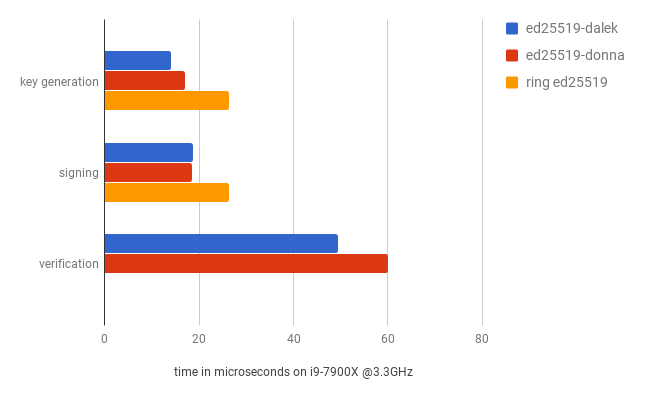
\includegraphics[height=7cm]{chart.png}
    \end{center}

  \end{frame}

  %% \begin{frame}
  %%   \frametitle{Rust features which could be better}
  %%   \begin{itemize}
  %%     \item The \alert{Eye of Sauron} \pause \texttt{\&(\&(\&(\&())))}
  %% 
  %%       \pause
  %%       Rust's operator traits take arguments of type \texttt{T}, not of type \texttt{\&T}.
  %% 
  %%       \pause To avoid a copy/move on every operation, you need to implement \texttt{Mul} for \texttt{\&T} instead of \texttt{T}:
  %% 
  %%       \pause {\small\texttt{let u = \&Z.square() - \&(\&constants::d4 * \&ss);}}
  %%       
  %%       \pause This gets messy quickly.  Possible solution: auto-borrow \texttt{Copy} types?
  %%       
  %%   \pause \item \alert{const generics!}
  %%       
  %%       \pause We've already thought of cool ways to abuse const generics to optimize field arithmetic.
  %%       
  %%       \pause Basic idea: statically track the sizes of intermediate values, and use specialization to insert reductions only when necessary.
  %% 
  %%   \end{itemize}
  %% \end{frame}
  
\section{Implementing cryptography with \texttt{-dalek}}

  %% \begin{frame}
  %%   \frametitle{\texttt{macros\_rule!} and zero-knowledge proofs}
  %%   
  %%   \alert{Zero-knowledge proofs} allow users to prove statements about secret values without revealing any extra information.
  %% 
  %%   \pause Example: given points $A, B, G, H$, and a secret value $x$, I want to prove that $A = Gx$ and $B = Hx$ without revealing anything about my secret $x$ value.
  %% 
  %%   \pause Implementing these proofs involves a lot of boilerplate, especially for proving more complicated expressions in zero knowledge.
  %%   
  %%   \pause \alert{Solution}: our \texttt{zkp} crate has an experimental zero-knowledge proof compiler in Rust macros.
  %%   
  %%   \pause {\small \texttt{create\_nipk!\{dleq, (x), (A, B, G, H) : A = (G * x), B = (H * x) \}} }
  %% 
  %%   \pause This creates a \texttt{dleq} module with all the code for creating and verifying these proof statements, using Serde to convert to/from wire format.
  %% \end{frame}
  
  \begin{frame}
    \frametitle{Implementing EdDSA signatures in \texttt{ed25519-dalek}}

    To create an EdDSA signature on a message, $m$, we first generate
    our keypair $(sk, pk)$ by choosing the secret scalar,
    $sk \uniformsample \ZZ / 2^{32}\ZZ$, that is, a random 32-byte
    string. \pause

    \begin{center}
      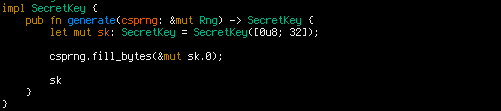
\includegraphics[height=3cm]{keygen-secret.png}
    \end{center}
  \end{frame}

  \begin{frame}
    \frametitle{Implementing EdDSA signatures in \texttt{ed25519-dalek}}

    We then hash $sk$ (RFC8032 specifies SHA-512), take the lower 256
    bits of the digest, reduce it as a scalar $x \in \ZZ / \ell\ZZ$,
    and then compute the public key as a point on the curve,
    $pk \gets x B$ where $B$ is the distinguished basepoint. \pause

    \begin{center}
      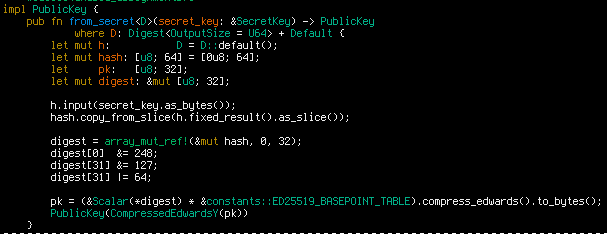
\includegraphics[height=5cm]{keygen-public.png}
    \end{center}
  \end{frame}


 \begin{frame}
   \frametitle{Implementing EdDSA signatures in \texttt{ed25519-dalek}}
 
   To sign the message $m$, we ``expand'' $sk$ by hashing it and reduce the low
   256-bits to a scalar $\texttt{sk\_expanded} \in \ZZ / \ell\ZZ$.  We then hash
   the concatenation of the high 256-bits of the digest and the message, and
   reduce the resulting digest into a scalar $r_0 \in \ZZ/\ell\ZZ$ which we
   multiply by the basepoint to produce the point $r \gets r_0 \times B$.
   
   Next, because relying on the sanctity of hash functions is an enormously
   appropropriate model for real world scenarios, we now compress $r$ into its
   Edwards y-coordinate (as a 32-byte array).  We concentenate the compressed
   form with the public key (also compressed), as well as --- again --- the
   message. The output digest is again reduced as a scalar
   $\texttt{hram\_digest} \in \ZZ/\ell\ZZ$.
   
   Finally, we compute
   $s \gets \texttt{hram\_digest} \times \texttt{sk\_expanded} + r_0$ and
   $t$ as the compressed Edwards y-coordinate of $r$.
   
   The signature now consists of 32 bytes of $t$ concatenated with 32 bytes of
   $s$.
 \end{frame}
 
 \begin{frame}
   \frametitle{Implementing EdDSA signatures in \texttt{ed25519-dalek}}
 
   \begin{center}
     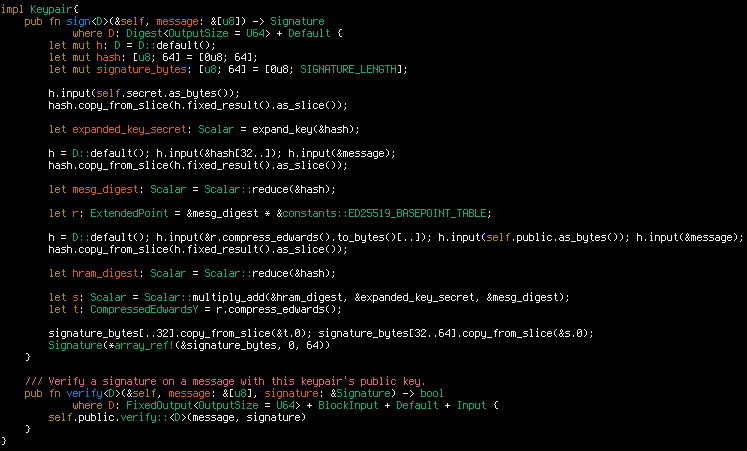
\includegraphics[height=7cm]{signing.png}
   \end{center}
 \end{frame}

 \begin{frame}
   \frametitle{Implementing EdDSA signatures in \texttt{ed25519-dalek}}

   For signature verification, 

 \end{frame}

 \begin{frame}
   \frametitle{Implementing EdDSA signatures in \texttt{ed25519-dalek}}
 
   \begin{center}
     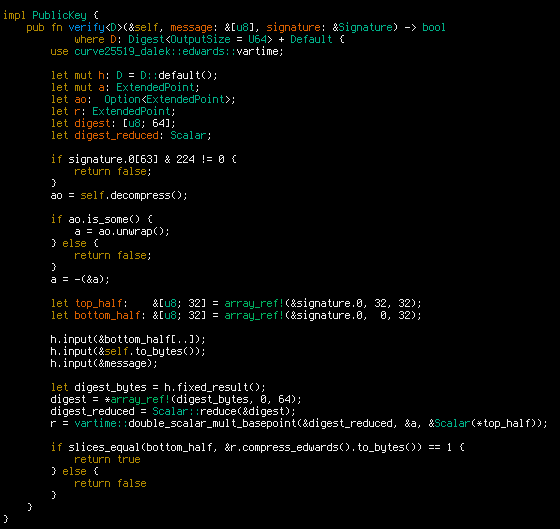
\includegraphics[height=7cm]{verification.png}
   \end{center}
 \end{frame}

 \begin{frame}
    \begin{center}
      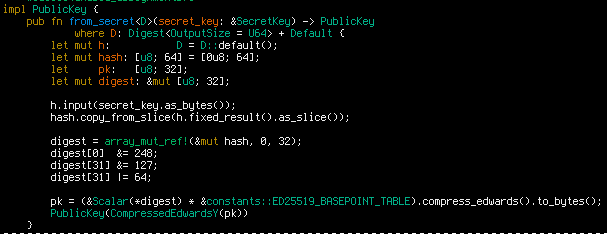
\includegraphics[height=5cm]{keygen-public.png}
    \end{center}
  \end{frame}

  \begin{frame}
    \frametitle{Implementing EdDSA signatures in \texttt{ed25519-dalek}}

    To sign the message $m$, we ``expand'' $sk$ by hashing it and
    reduce the low 256-bits to a scalar
    $\texttt{sk\_expanded} \in \ZZ / \ell/ZZ$.  We then hash the concatenation
    of the high 256-bits of the digest, the public key (compressed to only the Edwards
    y-coordinate, as an array of 32 bytes), and the message, and
    reduce the resulting digest into a scalar $r_0 \in \ZZ/\ell\ZZ$

  \end{frame}


  \begin{frame}
    \frametitle{Implementing rangeproofs with \texttt{-dalek}}
    
    Another type of zero-knowledge proof is a \alert{rangeproof}:
    proving that a secret number lies in a particular range, without
    revealing any other information.
    
    \pause These are used in confidential transaction systems, and in
    a future anti-censorship system we designed for Tor, called Hyphae.
    
    \pause Basic idea: to prove $x \in [0, b^n]$, write $x$ in base
    $b$ as $x = \sum_{i=0}^{n-1} x_i b^i$, and prove that each digit
    is in range: $x_i \in [0,b]$.
    
    \pause Verification essentially amounts to checking each digit's
    proof: if each digit is in range, the whole number is in range.
    
    \pause We implemented the Back-Maxwell rangeproof, which uses
    $b=3$ and shares data between digits to save space.
  \end{frame}

\begin{frame}[fragile]
    \frametitle{Implementing rangeproofs with \texttt{-dalek}: (partial) code}
    {\tiny
    \begin{minted}{rust}
    // mi_H[i] = m^i * H = 3^i * H in the loop below, construct these serially here:
    let mut mi_H = vec![*H; n];
    let mut mi2_H = vec![*H; n];
    for i in 1..n {
        mi2_H[i-1] = &mi_H[i-1] + &mi_H[i-1];
        mi_H[i] = &mi_H[i-1] + &mi2_H[i-1];
    }
    mi2_H[n-1] = &mi_H[n-1] + &mi_H[n-1];

    // Need to collect into a Vec to get par_iter()
    let indices: Vec<_> = (0..n).collect();
    let compressed_Ris: Vec<_> = indices.par_iter().map(|j| {
        let i = *j;

        let Ci_minus_miH = &self.C[i] - &mi_H[i];
        let P = vartime::multiscalar_mult(&[self.s_1[i], -&self.e_0], &[G, Ci_minus_miH]);
        let ei_1 = Scalar::hash_from_bytes::<Sha512>(P.compress().as_bytes());

        let Ci_minus_2miH = &self.C[i] - &mi2_H[i];
        let P = vartime::multiscalar_mult(&[self.s_2[i], -&ei_1], &[G, Ci_minus_2miH]);
        let ei_2 = Scalar::hash_from_bytes::<Sha512>(P.compress().as_bytes());

        let Ri = &self.C[i] * &ei_2;

        Ri.compress()
    }).collect();
    \end{minted}
    }
\end{frame}

\begin{frame}
  \frametitle{Cryptographic implementations we've made using \texttt{curve25519-dalek}}

  \begin{itemize}
    \pause \item \begin{tabular}{lr}
      \texttt{ed25519-dalek} & \href{https://github.com/isislovecruft/ed25519-dalek}{https://github.com/isislovecruft/ed25519-dalek}
      \end{tabular} \\
      EdDSA signatures in pure Rust.
    \pause \item \begin{tabular}{lr}
      \texttt{x25519-dalek} & \href{https://github.com/isislovecruft/x25519-dalek}{https://github.com/isislovecruft/x25519-dalek}
      \end{tabular} \\
      X25519 elliptic curve Diffie-Hellman(-Merkle) key exchange
    \pause \item \begin{tabular}{lr}
      \texttt{dalek-rangeproofs} & \href{https://github.com/isislovecruft/dalek-rangeproofs}{https://github.com/isislovecruft/dalek-rangeproofs}
      \end{tabular} \\
      Back-Maxwell rangeproofs using Borromean Ring signatures
    \pause \item \begin{tabular}{lr}
      \texttt{dalek-credentials} & \href{https://github.com/hdevalence/dalek-credentials}{https://github.com/hdevalence/dalek-credentials}
      \end{tabular} \\
      Algebraic Message Authentication Code (aMAC) and an algebraic-MAC-based,
      efficient, centralised issuer/verifier, anonymous credential scheme.
    \pause \item \begin{tabular}{lr}
      \texttt{zkp} & \href{https://github.com/hdevalence/zkp}{https://github.com/hdevalence/zkp}
      \end{tabular} \\
      A DSL resembing Camenisch-Stadler notation for proving statements about
      discrete logarithms in the Decaf group on curve25519
  \end{itemize}

\end{frame}


  \begin{frame}
    \frametitle{Thank you!}
    \begin{tabular}{ll}
      Isis Agora Lovecruft (speaker) & Henry de Valence (dalek coauthor)\\
      @isislovecruft                 & @hdevalence \\
      isis@patternsinthevoid.net     & hdevalence@hdevalence.ca \\
      https://patternsinthevoid.net  & https://hdevalence.ca
    \end{tabular}
  \end{frame}

\end{document}
